%************************************************
\chapter{Experimentation and Results}\label{ch:res}
As stated in Chapter \ref{ch:workflow}, each experiment was based on an hypothesis formulated after the observation of previous results. The structure of this chapter reflects this methodology.

Four experiments have been carried out, with more than 15 executions per experiment. Table \ref{t:resOver} shows an overview of the results.
\begin{table}[H]
	\myfloatalign
	\begin{tabularx}{\textwidth}{XXXXX} \toprule
		& \textbf{E1} & \textbf{E2} & \textbf{E3} &\textbf{E4} \\ \midrule
		\textbf{Time (h)} & 0.89 & 1.002 & 1.76 & 5.03 (h) \\ \midrule
		\textbf{G} &  100.0 & 155.087 & 76.625 & 365.929 \\ \midrule
		\textbf{Best} & 61.334 & 110.66 & 0.0015 & 0.0018 \\ \midrule
		\textbf{Avg} & 383.701 & 327.547 & 0.54 &  0.203 \\ \midrule
		\textbf{Worst}  & 510.515 & 367.895 & 0.828 & 0.2997\\ \midrule

		\bottomrule
	\end{tabularx}
	\caption{Summary of results, G: number of generations}
	\label{t:resOver}
\end{table}
% Experiment 1  & 3218.3255659076904 (s) & 100.0 & 61.334014263388944 & 383.70145875829604 & 510.51545656098943 \\ \midrule
% Experiment 2  & 3608.760242296302 (s) & 155.08695652173913 & 110.65943655439273 & 327.5473432160538 & 367.8950258239622 \\ \midrule
% Experiment 3  & 6348.083847716451 (s) & 76.625 & 0.0015238975513606394 & 0.539524085595754 & 0.8277429596344146 \\ \midrule
%Experiment 3  & 18116.758521642005 (s) & 365.92857142857144 & 0.001873980970385284 & 0.20283944348892707 & 0.2996970995967967 \\ \midrule

\section{First Experiment}
\subsection{Hypothesis}
The premise of this experiment is that our basic \acs{EA} should be able to minimize the movement of the blocks placed on the level and the flexibility of the representation should allow variety in the structures. This may be optimistic, but we need an estimation as a starting point, and this experiment will serve the purpose. 
\subsection{Execution}
The \acs{EA} in this experiments uses:
\begin{itemize}
	\item  initialization with the discrete method described in section \ref{ga:init}
	\item  basic sample crossover in section \ref{ga:cross1}
	\item  all four mutations (section \ref{ga:mut})
	\item  elitist replacement (section \ref{ga:rep})
	\item  selection using tournaments (section \ref{ga:select})
\end{itemize}

The parameters are:
\begin{itemize}
	\item Population size: 100
	\item Number of generations: 100
	\item Percentage of parents: 0.5
	\item Percentage of type mutations: 0.5
	\item Percentage of rotation mutations: 0.5
	\item Percentage of axis x mutations: 0.5
	\item Percentage of axis y mutations: 1
\end{itemize}
\subsection{Results}
The results suggest that the hypothesis was not correct. The average best solution has a fitness value of 61.334 (as shown in Table \ref{t:resOver}) which indicates that probably most levels have blocks falling (and even breaking) when loaded. The standard deviation of this measure is 133.0209 which implies that while some executions performed poorly, some others may be good. Some of the levels with lowest fitness value can be found in section \ref{a:e1}. Even those levels have blocks that break after loading so they would not be valid. However, we can tell there is variety in the structures, since they clearly differ from each other. 

In the experiment the only termination condition was reaching the maximum number of generations. However, looking at the results, it seems that the execution ended before the population stabilised or converged. Since mutation percentages are high it is normal that convergence where every single individual is the same one, is not reached. However, it could be possible that the population is stable, where every child has a grater fitness value than its parents, therefore no new members are allowed. If there is no new individuals and the population is completely \textit{stuck}, the fitness value of the worst individual should be the same over several generations. In Figure \ref{f:grahp1} we can see that is not the case in average. Although some populations do remain the same for several generations close to the maximum, most of them do not. 

\begin{figure}[H]
	\centering
	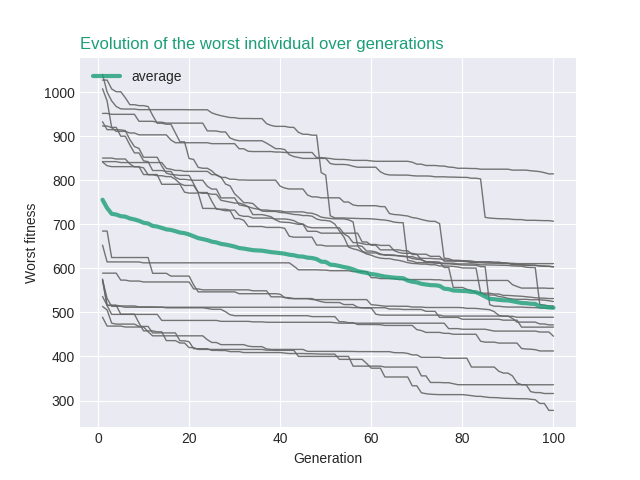
\includegraphics[scale=0.55]{gfx/exp1_worstIndv.png}
	\caption{In grey, different executions of the first experiment 1}\label{f:grahp1}
\end{figure}

% Aqui evolucion del peor individuo
\section{Second Experiment}
\subsection{Hypothesis}
Most executions from the previous experiment reached the maximum number of generations without stabilizing or converging. This means the \acs{EA} may need a larger number of generations to fully evolve a solution. 
\subsection{Execution}
The set of operators is the same as the previous one. The parameters remain unchanged except for:
\begin{itemize}
	\item Number of generations: 1000
\end{itemize}
We also added two stop conditions: 10 generations without changes (stable population) or best fitness value below 0.01.
\section{Results}
A sample of four of the levels generated can be found in the Appendix (\ref{a:e2}). Three of the levels were selected for having the lowest fitness value, but Figure \ref{f:e2-3} was visually interesting despite having a high fitness value due to a couple blocks broken on loading. 

Although best levels obtained with this experiment are better than those evolved in the first experiment, the bad solutions have a really high fitness value. In table \ref{t:resOver}, we can see that average fitness of levels produced with this version of the \acs{EA} is worse than the ones generated in the first experiment. It suggest that populations can be stuck for many generations before making any type of improvement. Any of the generated levels have a fitness below 0.01 or reached maximum number of generations, which means the termination criteria  that stopped the evolution was that the population was stable, without any new individuals added for 10 generations. 
\begin{figure}[H]
	\centering
	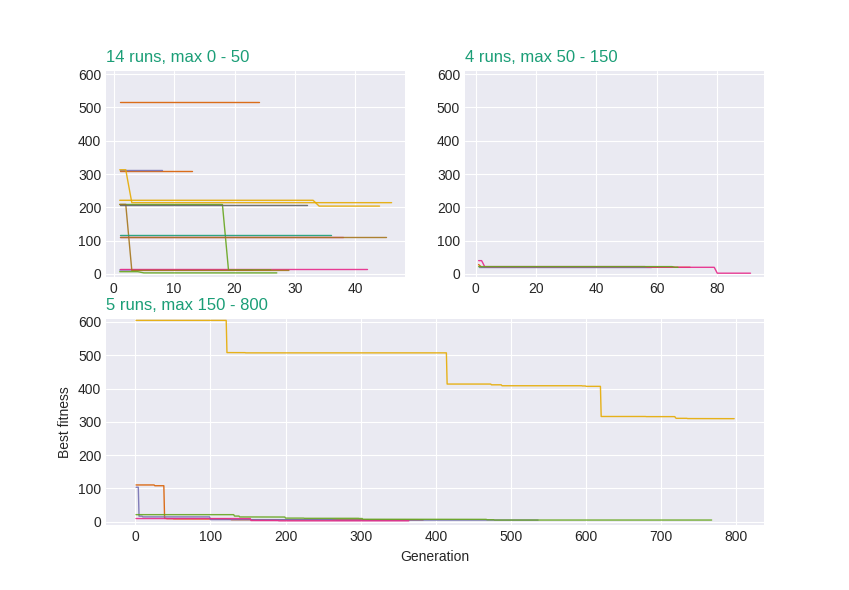
\includegraphics[scale=0.5]{gfx/exp2_explication.png}
	\caption{Best individual evolution for all executions, grouped by number of generations}\label{f:grahp2}
\end{figure}
Figure \ref{f:grahp2} represents the evolution of the best individual of each execution. Most of them have no more than 50 generations, therefore the hypothesis for this experiment is not correct. Short evolutions show that the best individual at initialization is very similar to the last one. Slight improvements may be achieved by small mutations but it seems difficult for new generations to outperform previous ones. We can appreciate that significant improvements are most common in those executions with a poor initial population. Even the ones with several hundreds of generations struggle to improve th intial population.

\section{Third Experiment}
\subsection{Hypothesis}
The previous experiment proved that the problem is not with the number of generations. Then it is more likely that there this \acs{EA} is biased towards exploration rather than exploitation. The genetic operators are failing to create new individuals that inherit good traits from their parents. A new crossover operator could shift the focus to exploitation.
\subsection{Execution}
This time the change introduced is in the crossover operator used. It was described in section \ref{ga:cross2}. The rest of the operators as well as the termination criteria are kept the same. 
\subsection{Results}
Table \ref{t:resOver} shows that the results have radically improved as the average fitness of the best solutions drops to 0.0015, a decrease of almost 100\%. Additionally, it took less generations in general to reach those results. However, executions took longer on average, which makes sense given that a greater number of individuals would have been simulated. The average fitness of the population and the worst individual have similar values now, which suggest that in most executions the population did converge. The Appendix section \ref{a:e4} contains four levels generated with this \acs{EA}. The selected levels are not necessarily the ones with less fitness value since with such small values the difference in stability is imperceptible.

The levels are stable and the blocks do not fall when loading the level, but they could arguably be considered structures, since most of them consist in a few blocks displayed on the floor. The average amount of blocks is 6.26, which is really close to the minimum amount of blocks allowed. However, given the proposed fitness function, it is completely logical that the evolution leads to this kind of arrangements. The more object placed on the level, the more likely the individual is to not meet the requirements imposed by the constraints. It also makes sense to place objects near the ground, instead of one on top of the other.
\section{Fourth Experiment}
\subsection{Hypothesis}
The previous \acs{EA} generates levels with a number of blocks that tends to the minimum of blocks allowed which is 5. Such a small number of elements does not create interesting structures. A higher number of blocks may lead to more appealing levels.
\subsection{Execution}
The only parameter that was changed for this experiment is the minimum number of blocks from 5 to 10. 
\subsection{Results}
The first thing to notice in these experiment(Table \ref{t:resOver}) is the increase of the average execution time: it went from 1.76 hours in the third experiment to 5.03 hours in this one. The time spent running the simulation for each population in this experiments and in the previous one should be similar. However, the number of executions drastically increased too. There is no doubt that placing at least ten objects is more difficult than placing 5. The average best fitness value slightly raised, while the average and worst values are lower. This suggest that the latest generations of this \acs{EA} are less diverse than those from the third experiment. 

Examples of the levels can be found in the Appendix section \ref{a:e4}. Even though levels are a little less stable this time, they are more interesting, which does not mean they could be considered fun levels, or levels at all.
%************************************************

%*****************************************
%*****************************************
%*****************************************
%*****************************************
%*****************************************
